\documentclass[11pt,letterpaper]{article}
\usepackage[T1]{fontenc}
\usepackage{lmodern,microtype,amsmath,amssymb,graphicx,booktabs,tabularx,array,enumitem,xcolor,fancyhdr,titlesec,tcolorbox,caption}
\tcbuselibrary{breakable}
\usepackage[margin=.8in,headheight=15pt,headsep=18pt,footskip=25pt]{geometry}
\usepackage[colorlinks=true,urlcolor=teal,linkcolor=olive]{hyperref}
\definecolor{olive}{HTML}{536240}\definecolor{ink}{HTML}{293329}\definecolor{teal}{HTML}{17677A}\definecolor{gold}{HTML}{A55C21}\definecolor{soft}{HTML}{EEF3E8}\definecolor{warm}{HTML}{FBEFDF}
\color{ink}\setlength{\parindent}{0pt}\setlength{\parskip}{7pt}
\setlist{leftmargin=1.4em,itemsep=3pt,topsep=3pt}
\renewcommand{\thesection}{4.\arabic{section}}
\titleformat{\section}{\Large\bfseries\color{olive}}{\thesection}{.6em}{}
\titleformat{\subsection}{\large\bfseries\color{teal}}{}{0pt}{}
\titlespacing*{\section}{0pt}{4pt}{12pt}\titlespacing*{\subsection}{0pt}{11pt}{4pt}
\pagestyle{fancy}\fancyhf{}\fancyhead[L]{\small\sffamily MATH\& 107 / WEEK 4}\fancyhead[R]{\small\sffamily Statistical Inference}\fancyfoot[L]{\small\sffamily Math in Society / Dr Lee}\fancyfoot[R]{\small\sffamily\thepage}\renewcommand{\headrulewidth}{.3pt}
\tcbset{boxrule=.5pt,arc=2mm,left=10pt,right=10pt,top=7pt,bottom=7pt,before skip=9pt,after skip=9pt,colframe=olive!35,colback=soft,fonttitle=\bfseries,coltitle=teal,colbacktitle=soft}
\newcolumntype{Y}{>{\raggedright\arraybackslash}X}
\captionsetup{font=small,labelformat=empty,textfont={color=teal},skip=7pt}
\hypersetup{pdftitle={Week 4: Statistical Inference},pdfauthor={MATH and 107 / Dr Lee}}
\usepackage{needspace}
\pdfinfoomitdate=1
\pdftrailerid{}
\pdfsuppressptexinfo=15
\setlength{\emergencystretch}{2em}

\widowpenalty=10000
\clubpenalty=10000

\begin{document}
{\small\sffamily\color{olive}WEEK 4 / NORMAL DISTRIBUTIONS AND STATISTICAL INFERENCE\par}
\vspace{12pt}
{\fontsize{30}{34}\selectfont\bfseries\color{olive}Individual variation\\and population estimates\par}
\vspace{10pt}
{\large Locate an individual measurement, describe a normal region, and interpret uncertainty in an estimate from a sample.\par}
\begin{center}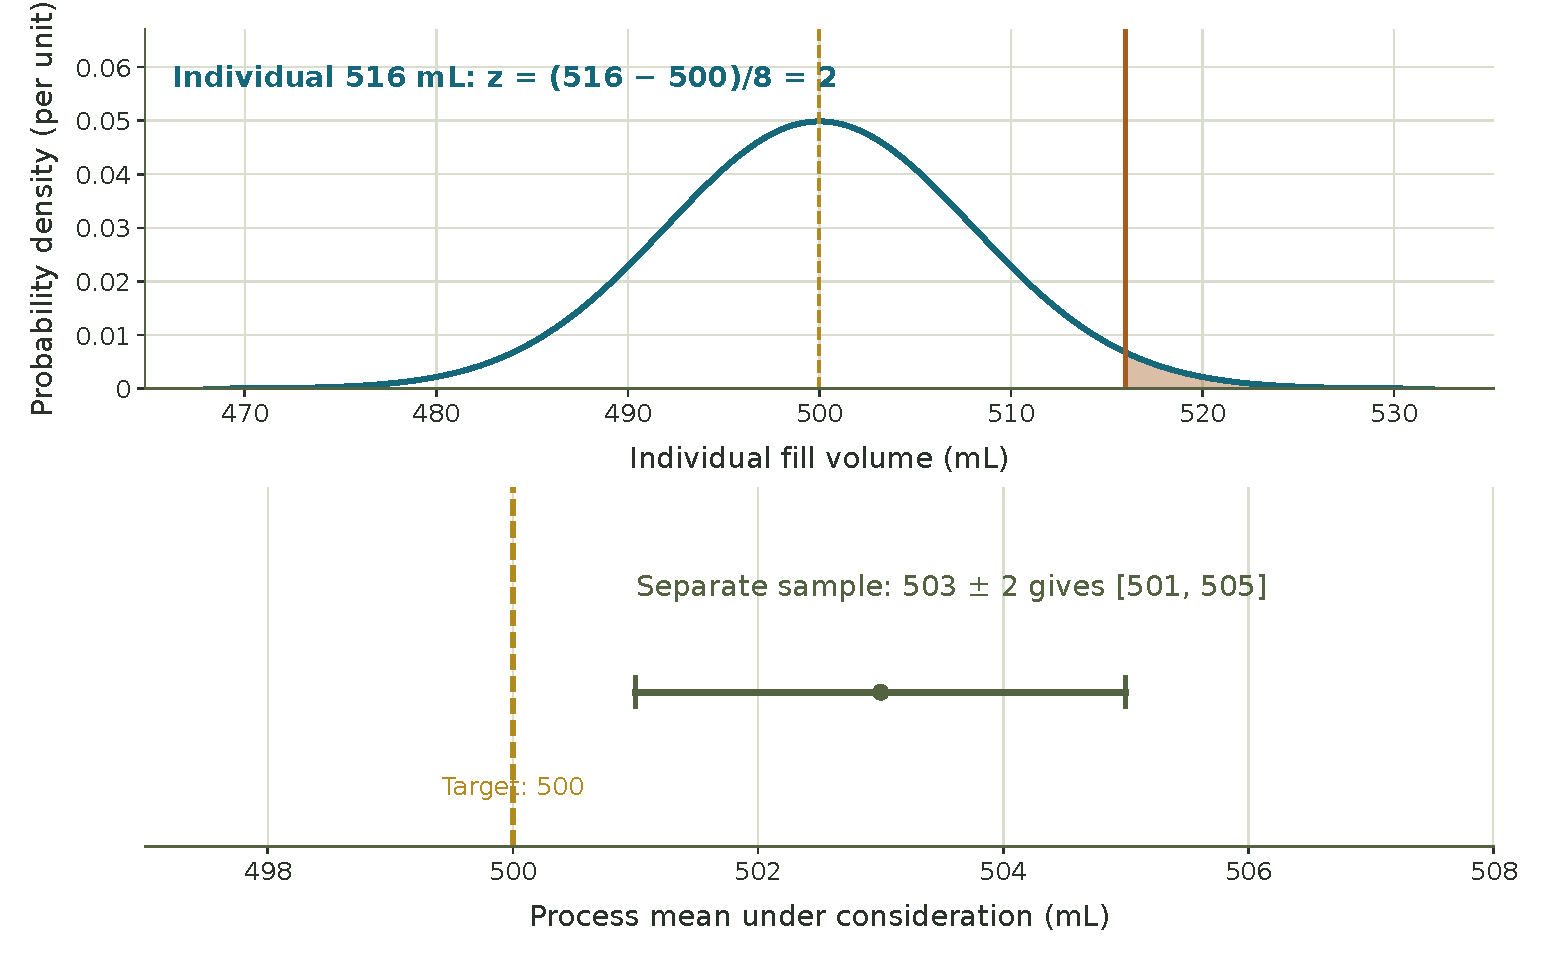
\includegraphics[width=\linewidth,height=3.15in,keepaspectratio]{../assets/week4/bottle-two-questions.pdf}\end{center}
\begin{tcolorbox}[title={Two questions about one process}]
A bottle at 516 mL is compared with a normal model centered at 500 mL with standard deviation 8 mL. A separate sample gives mean 503 mL and margin 2 mL. The first question concerns an individual bottle; the second concerns the process mean. A correct calculation must answer the intended question.
\end{tcolorbox}
Week 3 introduced center and spread. This chapter adds normal models, standardized position, sampling variability, and confidence intervals. Its core interval exercises supply their margins. The standard-error and repeated-sampling examples explain the meaning of those margins under stated assumptions.

Try the short checks before reading their explanations. Review exercises retain the principal numerical settings used in the course and include complete solutions. All examples are hypothetical.

\medskip
\href{https://bobovski66.github.io/MathInSociety/readings/week4_reading.html}{Online reading}\quad\textperiodcentered\quad\href{https://bobovski66.github.io/MathInSociety/demos/normal_z.html}{Statistical explorer}\quad\textperiodcentered\quad\href{https://bobovski66.github.io/MathInSociety/labs/week4_lab.html}{Laboratory}
\clearpage


\Needspace{6\baselineskip}\section{Normal shape, center, and spread}

A histogram summarizes the frequencies of measurements. Some histograms have a roughly symmetric mound: most measurements are near the center, and increasingly fewer lie far away on either side. A \emph{normal distribution} is a smooth mathematical model of that shape. It is a model to consider, rather than a shape every dataset must have.


The mean \(\mu\), pronounced ``mu,'' gives the center. The standard deviation \(\sigma\), pronounced ``sigma,'' gives the spread in the same units as the measurements. The model requires \(\sigma>0\). When the standard deviation is larger, values spread over a wider range. A narrower normal curve is taller because the total area under either curve is 1, representing 100\% of possible outcomes.


\par\medskip\noindent\begin{minipage}{\linewidth}
\centering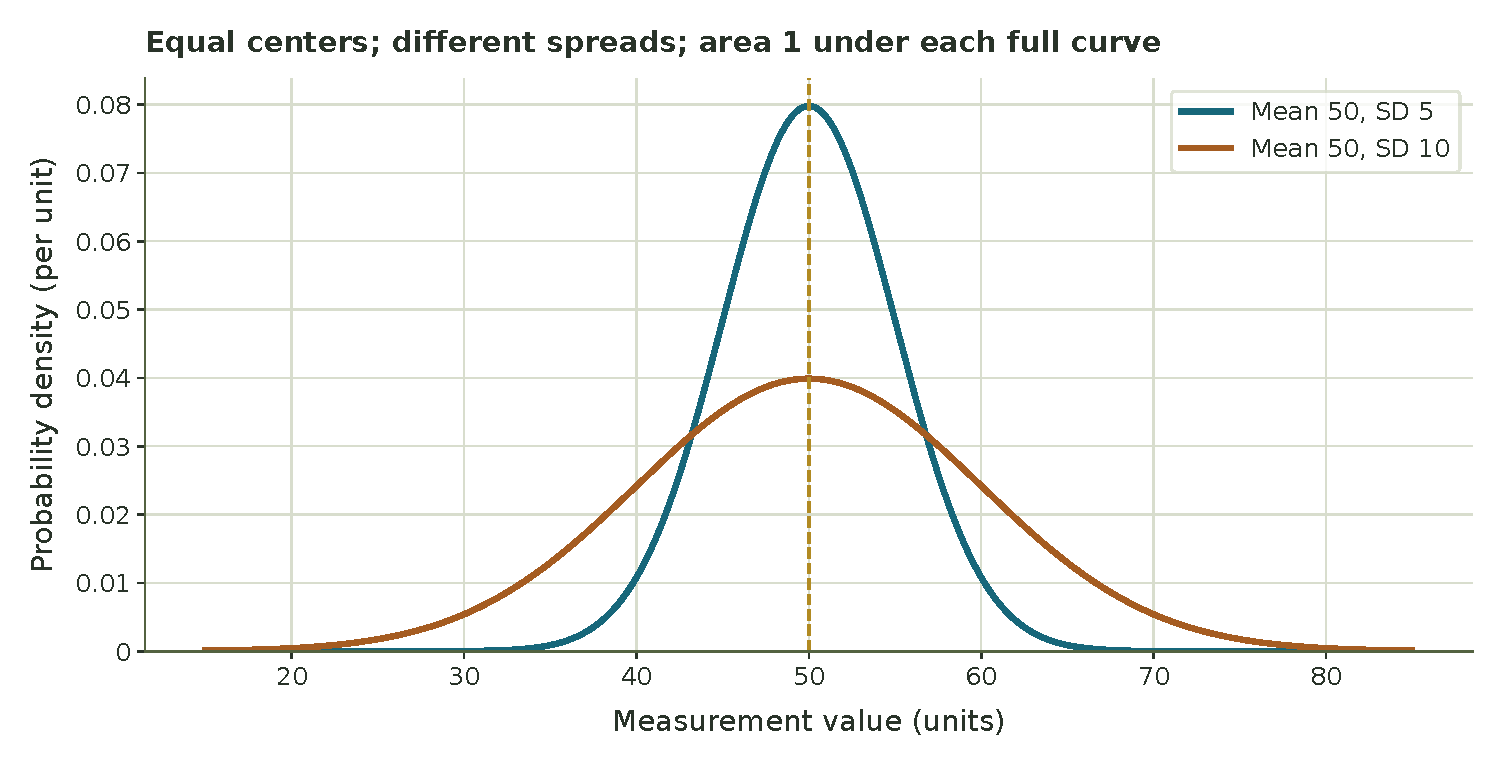
\includegraphics[width=\linewidth,height=2.8in,keepaspectratio]{../assets/week4/normal-shape.pdf}
\captionof*{figure}{Mean locates the center; standard deviation changes the spread. Probability belongs to an area over a range, not to the height at one point.}
\end{minipage}\par\medskip

For a continuous measurement, the probability of a range is represented by the area under the curve over that range. The curve's height is \emph{density}, not a percentage. Mean, median, and the peak coincide in a normal distribution because it is symmetric and has one peak.


Here we specify a normal model by naming its mean and standard deviation. If we use the notation \(N(\mu,\sigma^2)\), its second entry is the \emph{variance}, the square of the standard deviation. Naming both quantities avoids a notation ambiguity found across textbooks.


Before using a normal model, consider the shape and context of the data. Waiting times can have a long right tail; a mixture of two groups can have two peaks. Real measurements may also have bounds that the ideal normal curve does not. Check whether the model is a reasonable approximation for the question and range of interest.


\begin{tcolorbox}[title={Pause and try 1},breakable]
Two approximately normal processes have the same mean but different standard deviations. Which has the wider central range of measurements?
\end{tcolorbox}

\clearpage

\Needspace{6\baselineskip}\section{The Empirical Rule}

For an approximately normal distribution, the Empirical Rule gives three useful approximations. About 68\% of values lie within one standard deviation of the mean, about 95\% within two, and about 99.7\% within three. ``Within'' includes values on both sides of the center.

\[\mu-k\sigma\ \text{ to }\ \mu+k\sigma.\]
First choose the number of standard deviations k. Multiply the standard deviation by k, then subtract and add that distance from the mean. The resulting endpoints have the original measurement units.


\par\medskip\noindent\begin{minipage}{\linewidth}
\centering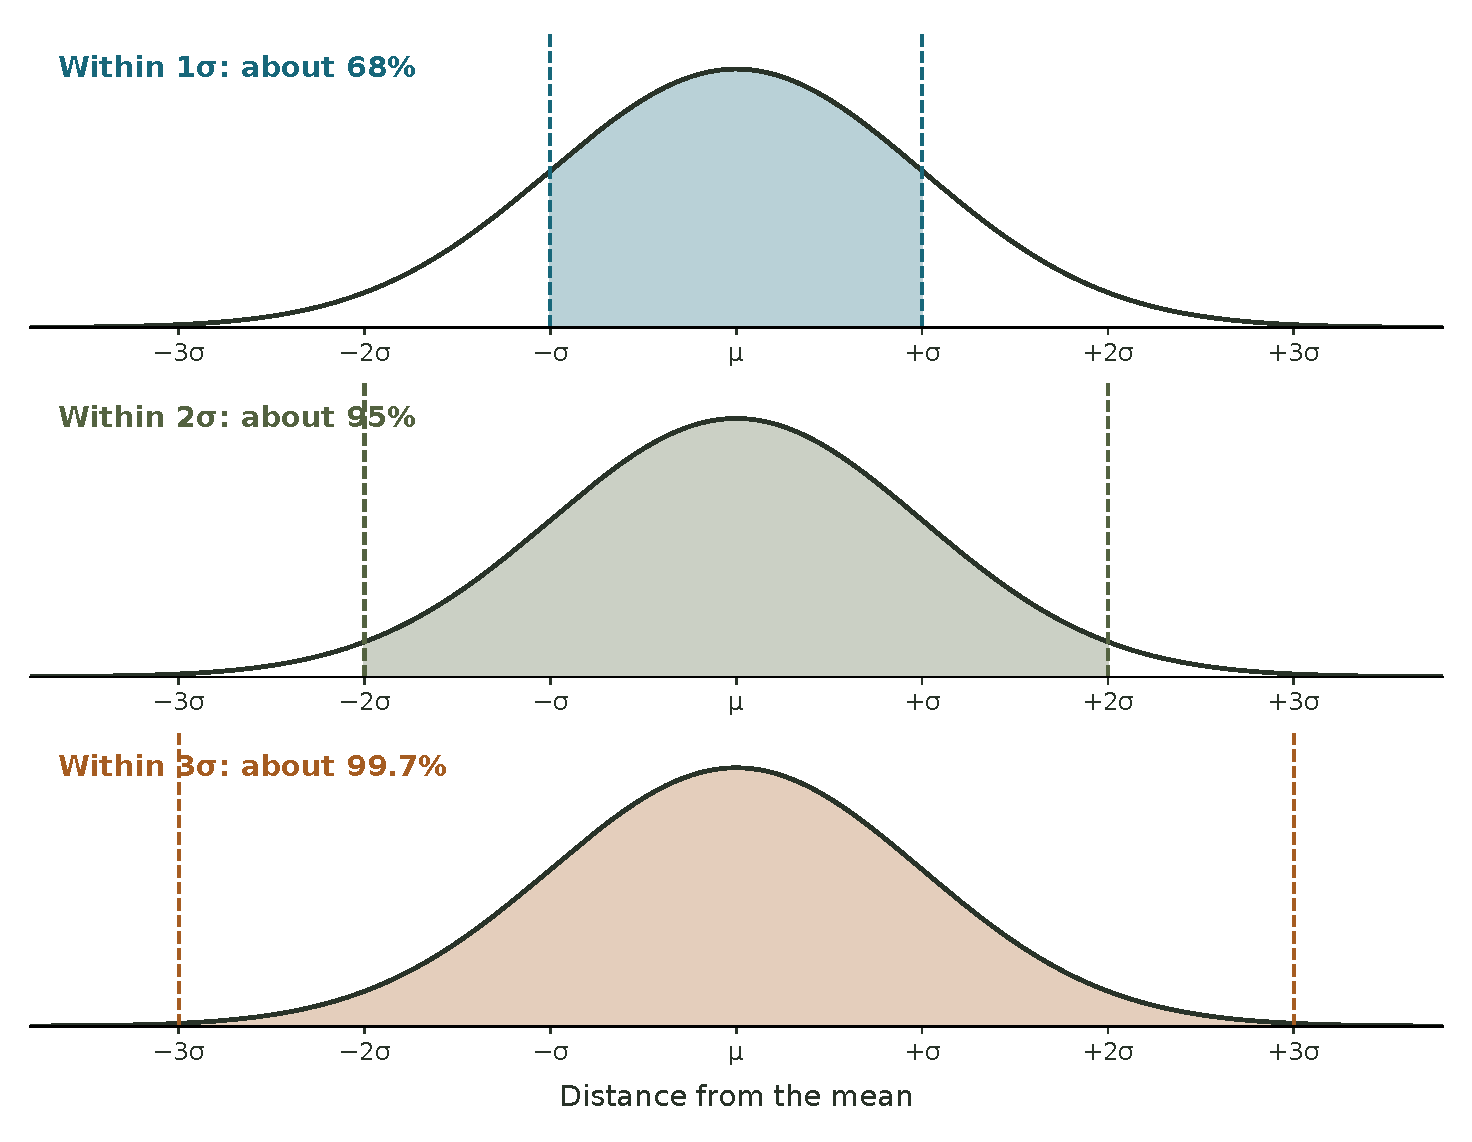
\includegraphics[width=\linewidth,height=4.7in,keepaspectratio]{../assets/week4/empirical-bands.pdf}
\captionof*{figure}{These are three nested central regions. The 95\% region includes the inner 68\%; the percentages are not three separate slices to add.}
\end{minipage}\par\medskip

\begin{tcolorbox}[title={Delivery times},breakable]

Suppose delivery times are approximately normal with mean 30 minutes and standard deviation 4 minutes. The central intervals are:


\par\medskip{\small\renewcommand{\arraystretch}{1.35}\begin{tabularx}{\linewidth}{@{}YYYY@{}}\toprule
Distance from mean & Calculation & Interval & Approximate share\\
\midrule
1 standard deviation & 30 $\pm$ 4 & 26--34 minutes & 68\%\\
2 standard deviations & 30 $\pm$ 8 & 22--38 minutes & 95\%\\
3 standard deviations & 30 $\pm$ 12 & 18--42 minutes & 99.7\%\\
\bottomrule\end{tabularx}}\par\medskip

If we observed 1,000 deliveries from this model, about 950 would fall between 22 and 38 minutes on average. A particular collection need not contain exactly 950. The rule describes a model proportion, not a guarantee about a finite count.


\end{tcolorbox}

\begin{tcolorbox}[title={Pause and try 2},breakable]
A normal model has mean 50 and standard deviation 6. Find the interval containing about 95\% of individual values.
\end{tcolorbox}


\Needspace{6\baselineskip}\section{Complements and the two tails}

If about 95\% of values lie in the central region, the remaining 5\% lie outside it. A normal curve is symmetric, so the two tails contain equal shares: about 2.5\% below \(\mu-2\sigma\) and 2.5\% above \(\mu+2\sigma\).


\par\medskip\noindent\begin{minipage}{\linewidth}
\centering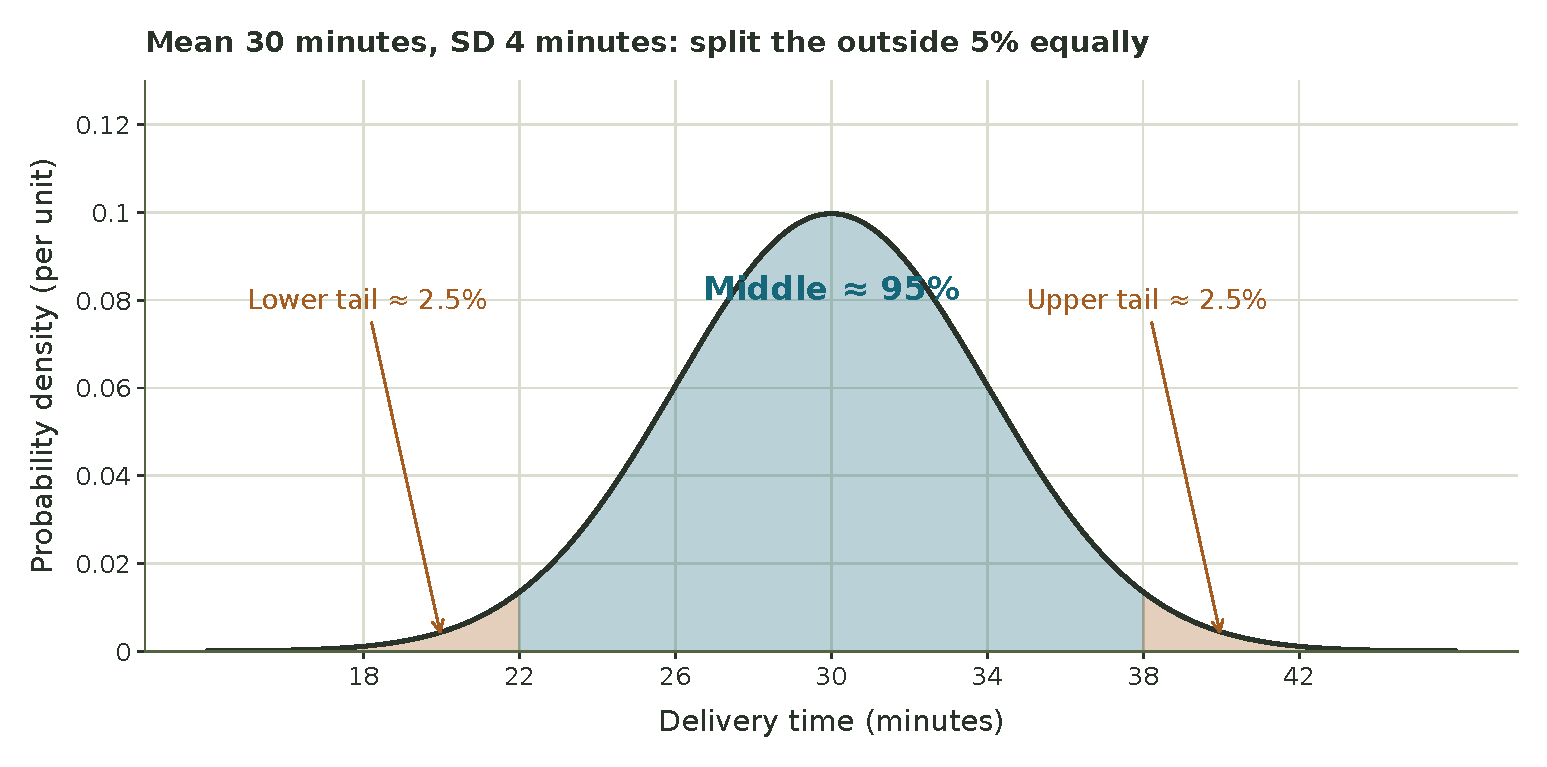
\includegraphics[width=\linewidth,height=2.8in,keepaspectratio]{../assets/week4/empirical-tails.pdf}
\captionof*{figure}{Take the complement first, then divide between the two tails. ``Above 38'' is one tail; ``outside 22--38'' includes both.}
\end{minipage}\par\medskip

\par\medskip{\small\renewcommand{\arraystretch}{1.35}\begin{tabularx}{\linewidth}{@{}YYYY@{}}\toprule
Boundary & Central share & Outside both sides & One tail\\
\midrule
$\mu$ $\pm$ $\sigma$ & 68\% & 32\% & 16\%\\
$\mu$ $\pm$ 2$\sigma$ & 95\% & 5\% & 2.5\%\\
$\mu$ $\pm$ 3$\sigma$ & 99.7\% & 0.3\% & 0.15\%\\
\bottomrule\end{tabularx}}\par\medskip

For the delivery example, about 16\% take longer than 34 minutes, and about 2.5\% take longer than 38 minutes. These are approximate Empirical Rule answers. A normal-distribution calculator gives slightly different, more precise values. Use the approximation requested by a question.


The rule does not directly give a percentage for every boundary. For example, a cutoff 1.9 standard deviations above the mean is between the one- and two-standard-deviation marks. The Empirical Rule alone does not supply its exact upper-tail probability.


\begin{tcolorbox}[title={Pause and try 3},breakable]
Approximately what percentage lies above one standard deviation above the mean? What percentage lies outside the central two-standard-deviation interval?
\end{tcolorbox}


\Needspace{6\baselineskip}\section{Z-scores and relative position}

A raw value becomes meaningful in relation to a center and a spread. A \emph{z-score} expresses a signed distance from the mean in standard-deviation units:

\[z=\frac{x-\mu}{\sigma},\qquad x=\mu+z\sigma.\]
Subtracting the mean finds the signed distance in the original units. Dividing by the standard deviation changes the unit of that distance. Positive means above the mean; negative means below; zero means at the mean. The original measurement units cancel, so z has no measurement unit.


\par\medskip\noindent\begin{minipage}{\linewidth}
\centering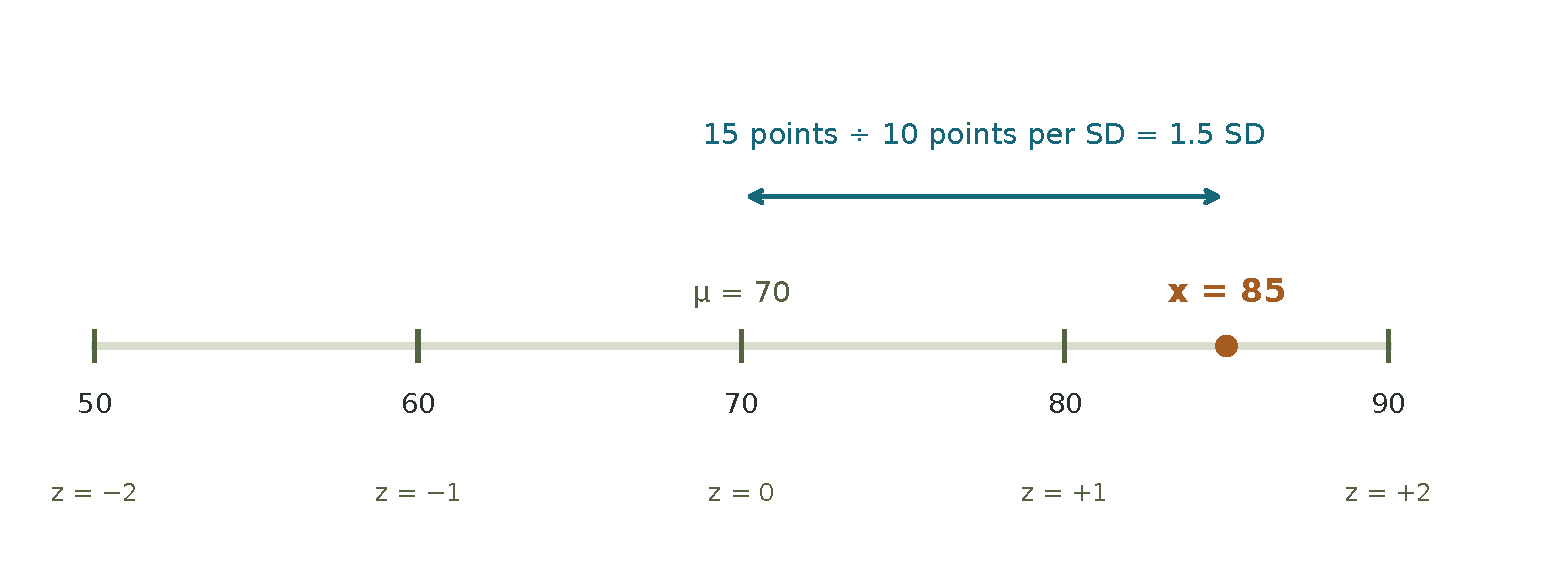
\includegraphics[width=\linewidth,height=2.8in,keepaspectratio]{../assets/week4/z-score-distance.pdf}
\captionof*{figure}{Read z = 1.5 as ``one and a half standard deviations above the mean,'' not as a probability of 1.5 or a 1.5-point difference.}
\end{minipage}\par\medskip

\begin{tcolorbox}[title={Calculate, interpret, then reverse},breakable]

With mean 70 and standard deviation 10, a value of 85 has \(z=(85-70)/10=1.5\). A value at z = $-$2 is \(x=70+(-2)(10)=50\). A negative z-score does not require a negative raw value.


\end{tcolorbox}

\par\medskip\noindent\begin{minipage}{\linewidth}
\centering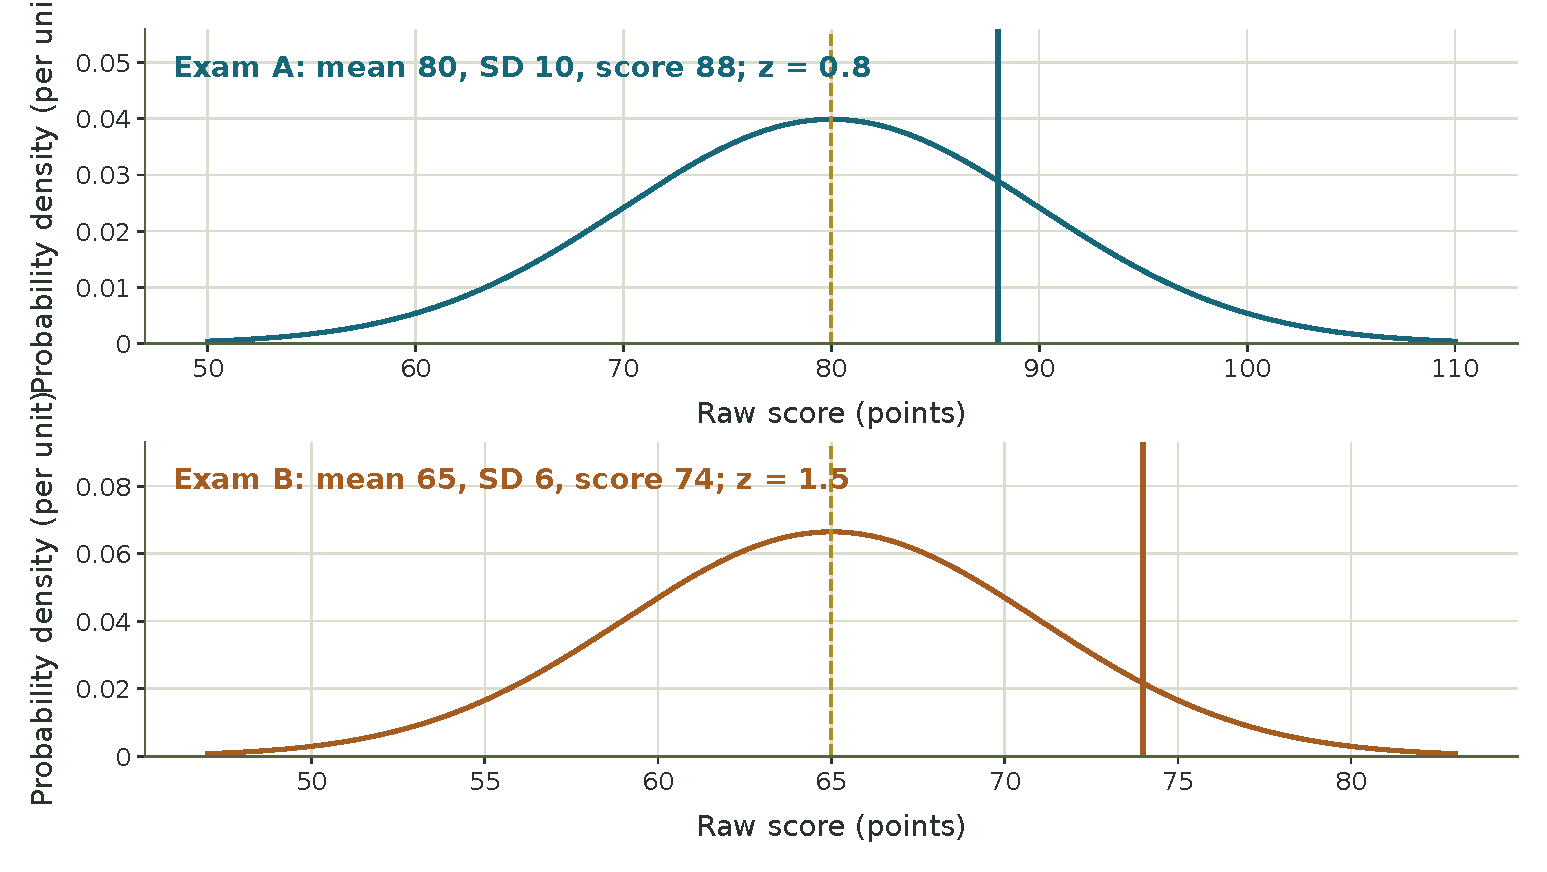
\includegraphics[width=\linewidth,height=3.35in,keepaspectratio]{../assets/week4/standardized-comparison.pdf}
\captionof*{figure}{The lower raw score is farther above its own group's mean. Standardization compares positions within distributions; it does not establish that different tests measure the same skill.}
\end{minipage}\par\medskip

For quantities such as completion times, a lower value may be preferred. A negative z-score can therefore describe a faster-than-average time. The sign locates a value; the context determines how to evaluate that location.


You can calculate a z-score for a distribution with a finite mean and positive standard deviation even if it is not normal. Normality matters when you use the bell curve or Empirical Rule to interpret percentages from that score.


\begin{tcolorbox}[title={Pause and try 4},breakable]
A value is 44 in a distribution with mean 50 and standard deviation 6. Find z. Then recover the raw value with z = 2 in that distribution.
\end{tcolorbox}

\clearpage

\Needspace{6\baselineskip}\section{Populations, samples, parameters, and statistics}

A \emph{population} is the entire collection the question concerns. A \emph{sample} is the subset actually observed. Define the population before collecting the sample: ``all boxes from this production process during this month'' is more specific than ``all cereal.''


\par\medskip{\small\renewcommand{\arraystretch}{1.35}\begin{tabularx}{\linewidth}{@{}YY@{}}\toprule
Population quantity: parameter & Observed sample quantity: statistic\\
\midrule
Mean $\mu$ of all units in the defined population & Mean \(\bar x\) calculated from the sample\\
Proportion p of all units with a property & Proportion \(\widehat p\) calculated from the sample\\
Standard deviation $\sigma$ of the population & Standard deviation s calculated from the sample\\
\bottomrule\end{tabularx}}\par\medskip

\begin{tcolorbox}[title={A campus survey},breakable]

A college wants the proportion of enrolled students who commute by bus. In a sample of 100 students, 34 answer yes. The sample proportion is \(\widehat p=34/100=0.34\), or 34\%. The unknown parameter is the proportion of all enrolled students who commute by bus. The sample size 100 is not that proportion.


\end{tcolorbox}

A mean describes a numerical measurement, such as fish length. A proportion describes the share satisfying a condition, such as using the bus. Both can be estimated from samples, but they are different parameters with different units.


How units are selected affects what the sample can represent. A simple random sample gives each subset of the specified size an equal chance of selection. A voluntary survey may overrepresent people who choose to respond. A large sample drawn from the wrong group does not automatically estimate the intended population well.


\begin{tcolorbox}[title={Pause and try 5},breakable]
A producer tests 100 batteries and finds a mean lifetime of 18.4 hours. Name the statistic, its target parameter, and the sample size.
\end{tcolorbox}


\Needspace{6\baselineskip}\section{Sampling variability and standard error}

If we selected another random sample, its members would usually differ, and so would its mean. That ordinary sample-to-sample variation is \emph{sampling variability}. Imagine repeating the whole procedure: select a sample, calculate a mean, record it, and start again with a new sample. The distribution of those recorded means is a \emph{sampling distribution}.


There are now two spreads to distinguish. The standard deviation of individuals describes differences among individual units. The \emph{standard error of the mean} describes how much the sample mean varies across repeated samples of the same size.


\par\medskip\noindent\begin{minipage}{\linewidth}
\centering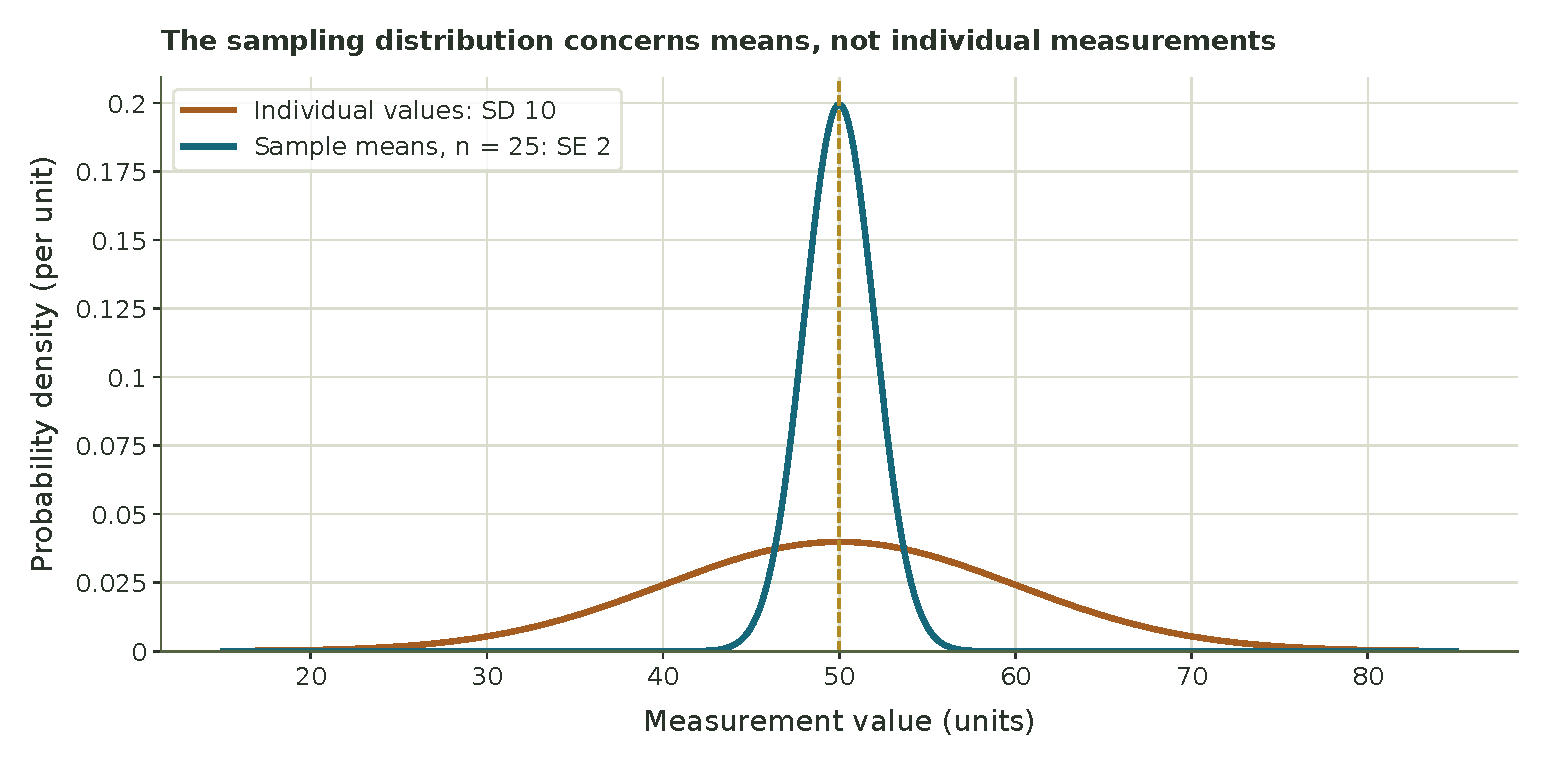
\includegraphics[width=\linewidth,height=2.8in,keepaspectratio]{../assets/week4/sampling-means.pdf}
\captionof*{figure}{Averages vary less than individual measurements. Taking more observations does not make the individual units themselves more alike.}
\end{minipage}\par\medskip

For independent, identically distributed observations with population standard deviation $\sigma$, the mean has standard error \(\sigma/\sqrt n\). When $\sigma$ is unknown, we often estimate that standard error with \(s/\sqrt n\). With $\sigma$ = 10 and n = 25, it is \(10/5=2\).


If the population is normal, its independent sample means are normal as well. For many other populations, an approximately normal sampling distribution can emerge as the sample grows, under the conditions of the central limit theorem. This does not make the original population normal. There is no sample size that automatically makes every sampling design and distribution suitable.


\begin{tcolorbox}[title={Pause and try 6},breakable]
Individual measurements have standard deviation 12 units. Under independent sampling, what is the standard error of a mean from n = 36? What stays at 12?
\end{tcolorbox}

\clearpage

\Needspace{6\baselineskip}\section{Interval estimates and comparison values}

A sample mean is a \emph{point estimate}. An interval estimate adds a margin of uncertainty. Most questions in this unit supply the margin of error E; your task is to construct and interpret the endpoints:

\[\text{estimate}-E\quad\text{to}\quad\text{estimate}+E.\]
\par\medskip\noindent\begin{minipage}{\linewidth}
\centering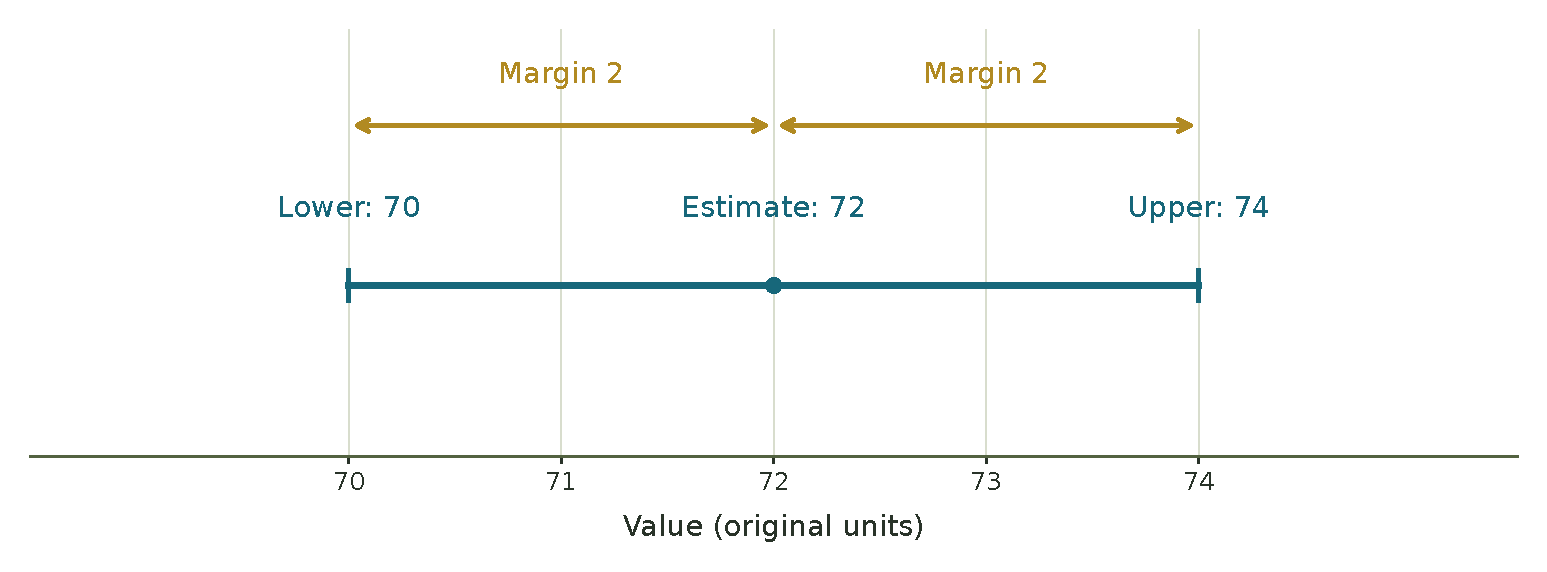
\includegraphics[width=\linewidth,height=2.8in,keepaspectratio]{../assets/week4/interval-anatomy.pdf}
\captionof*{figure}{Margin of error is the half-width. Keep the estimate, margin, endpoints, and full width in the same units.}
\end{minipage}\par\medskip

\begin{tcolorbox}[title={Hours and percentage points},breakable]

A mean estimate of 4.6 hours with margin 0.7 hours gives [3.9, 5.3] hours. A population proportion estimated at 54\% with margin 5 \emph{percentage points} gives [49\%, 59\%]. Subtracting 5\% of 54 would answer a different question.


\end{tcolorbox}

Compare a proposed parameter value with both endpoints. If it lies inside, including an endpoint, it is not excluded by this interval. That does not prove the proposed value is correct. If it lies outside, the interval excludes it under the method and assumptions used. That does not establish impossibility or explain what caused the discrepancy.


\par\medskip\noindent\begin{minipage}{\linewidth}
\centering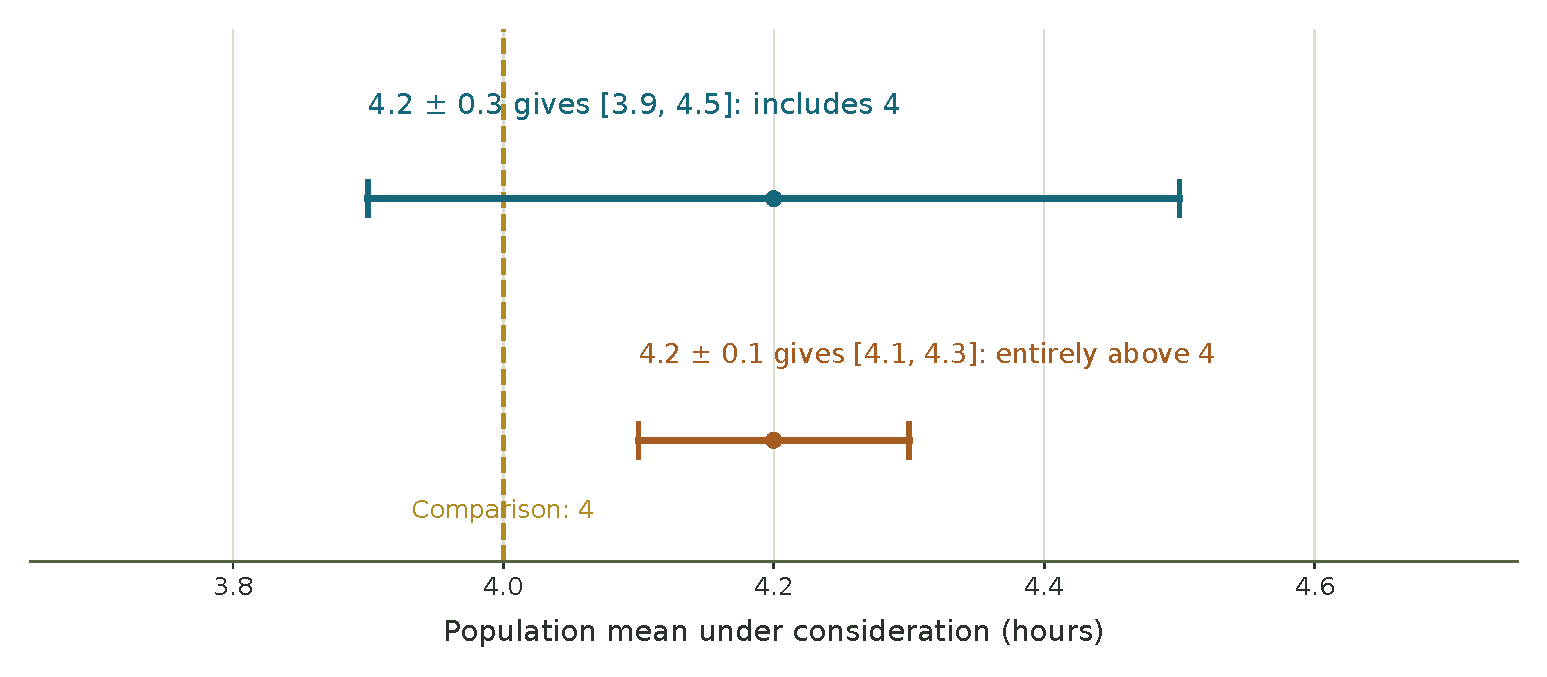
\includegraphics[width=\linewidth,height=2.8in,keepaspectratio]{../assets/week4/interval-comparisons.pdf}
\captionof*{figure}{The first interval allows population means below and above 4. Its sample estimate being above 4 does not put the entire interval above 4.}
\end{minipage}\par\medskip

The margin alone does not tell us a confidence level or validate a sampling procedure. A study should report how it obtained its interval. For a sufficiently large, appropriately sampled independent dataset, \(\bar x\pm2s/\sqrt n\) is a familiar rough 95\% mean interval. With mean 72, sample SD 10, and n = 100, this gives \(72\pm2\), or [70, 74]. More precise mean intervals commonly use a t multiplier when $\sigma$ is estimated.


\begin{tcolorbox}[title={Pause and try 7},breakable]
An estimate is 3.7 hours with margin 0.5 hours. Find the interval and decide whether 4 hours is excluded.
\end{tcolorbox}

\clearpage

\Needspace{6\baselineskip}\section{Interpreting a confidence level}

A 95\% confidence level describes the long-run coverage of a procedure. Imagine repeatedly taking samples by the same valid method and building an interval each time. About 95\% of those intervals would contain the fixed population parameter. The interval changes with the sample; the population parameter remains fixed in this picture.


\par\medskip\noindent\begin{minipage}{\linewidth}
\centering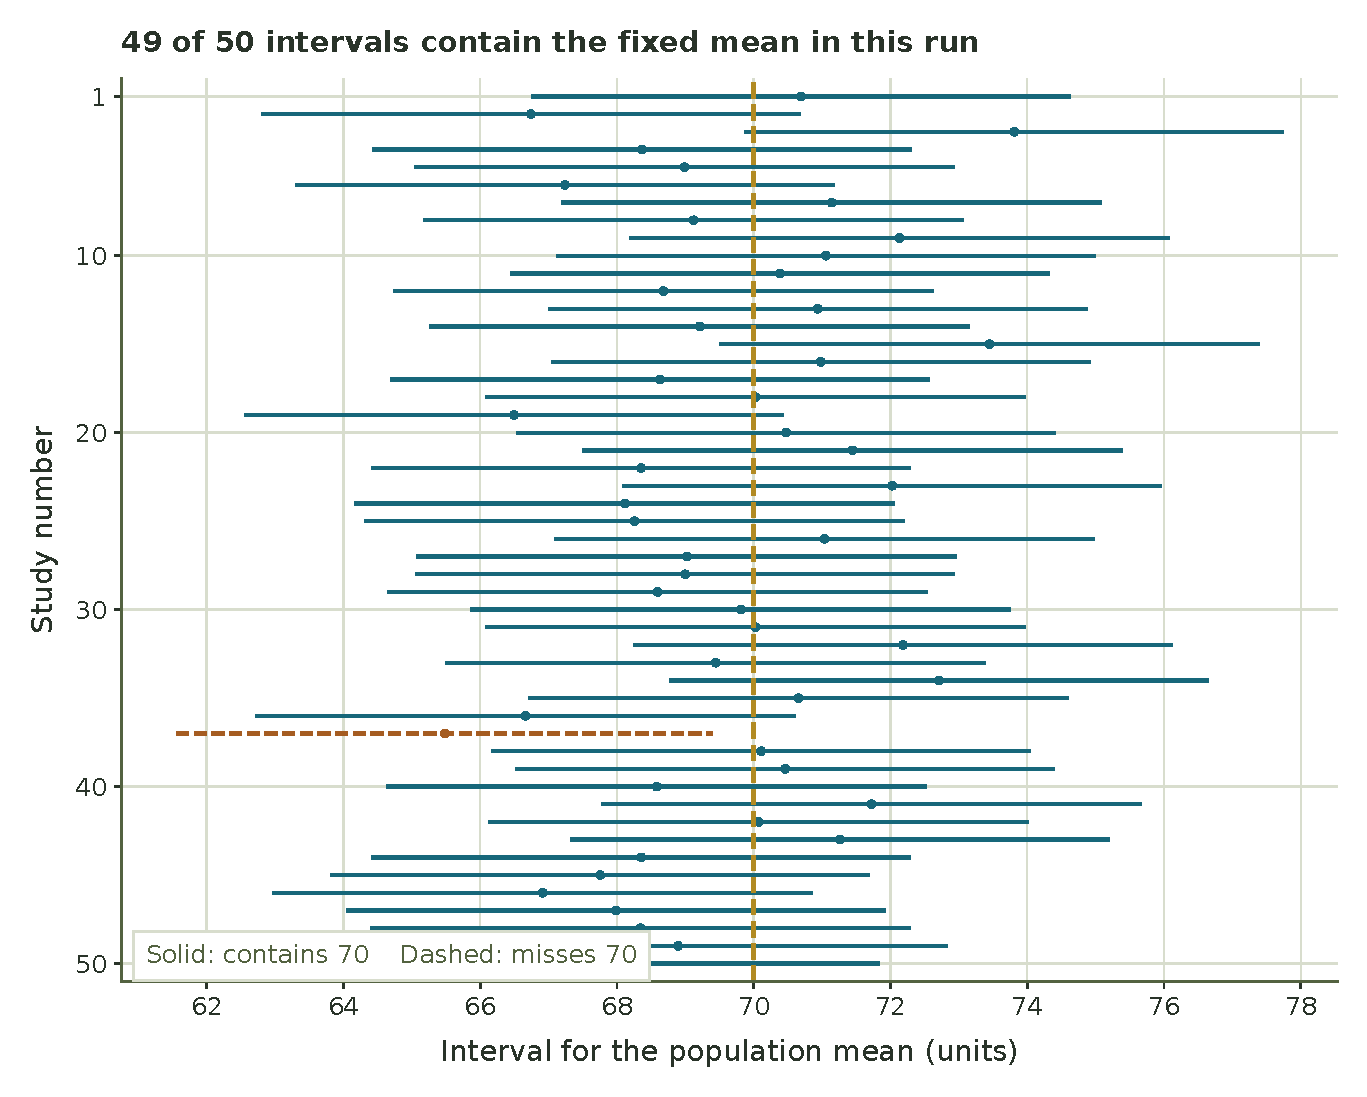
\includegraphics[width=\linewidth,height=4.1in,keepaspectratio]{../assets/week4/repeated-intervals.pdf}
\captionof*{figure}{An illustration using a normal population with known standard deviation. The observed coverage in a finite run need not be exactly 95\%.}
\end{minipage}\par\medskip

After one interval has been calculated, it either contains the fixed parameter or it does not. The confidence level does not mean 95\% of individual observations fall inside that interval, and it does not assign a 95\% probability to that one fixed parameter after the data are observed.


In the repeat-sampling experiment, the population mean is known because we chose the model. We can therefore check which intervals contain it. In an actual study, the unknown mean is precisely what we are trying to estimate.


For fixed data and the same method, seeking higher confidence generally requires a wider interval. A narrower interval is more precise, but its width alone does not establish that the study is representative or unbiased.


\begin{tcolorbox}[title={Pause and try 8},breakable]
A valid 95\% procedure is used for 50 independent samples. Must exactly 95\% of those 50 intervals contain the population mean?
\end{tcolorbox}


\Needspace{6\baselineskip}\section{Sample size, precision, and bias}

For comparable studies with the same confidence level, variability, and sampling design, margin of error often scales approximately as \(1/\sqrt n\). To compare a baseline study with a planned sample size, use

\[E_{\mathrm{new}}\approx E_0\sqrt{\frac{n_0}{n_{\mathrm{new}}}}.\]
If n changes from 100 to 400, the sample is four times as large but its square root is only twice as large. A baseline margin of 10 becomes approximately 5. To halve a margin, we need about four times the sample; to cut it to one-third, about nine times the sample.


\par\medskip\noindent\begin{minipage}{\linewidth}
\centering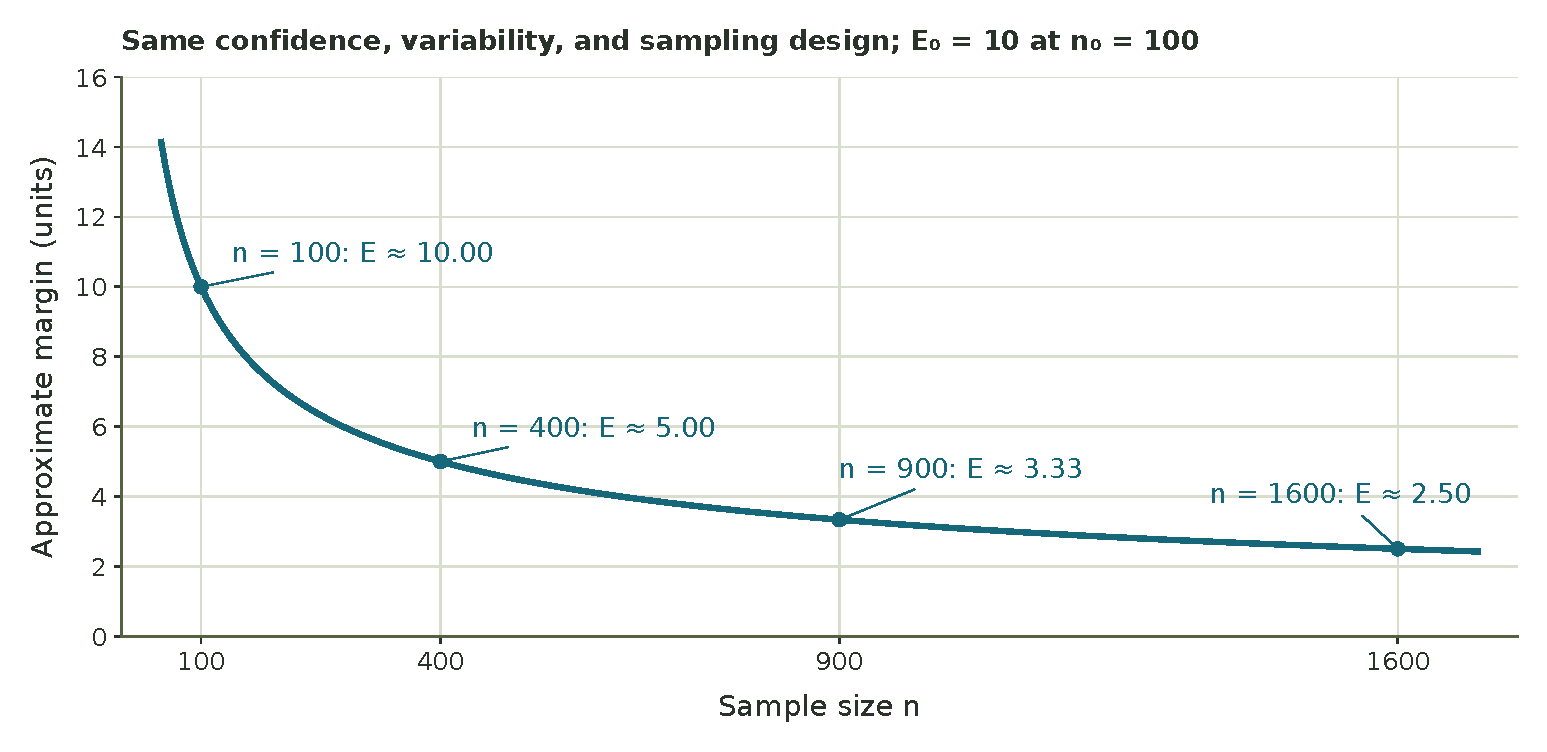
\includegraphics[width=\linewidth,height=2.8in,keepaspectratio]{../assets/week4/precision-scaling.pdf}
\captionof*{figure}{The improvement follows a square root, not a direct inverse of the sample size. It is a comparison under unchanged study conditions.}
\end{minipage}\par\medskip

These are planning comparisons. A larger actual sample can give a different mean, standard deviation, or estimated proportion, so its interval need not keep the old center or exactly match the planned width. The sample-size rule does not remove bias in selection or measurement, and correlated observations may provide less information than the same number of independent observations.


\begin{tcolorbox}[title={Pause and try 9},breakable]
A study has n = 200. Approximately what sample size would halve its margin under comparable conditions?
\end{tcolorbox}


\Needspace{6\baselineskip}\section{Choosing and interpreting a method}

\par\medskip{\small\renewcommand{\arraystretch}{1.35}\begin{tabularx}{\linewidth}{@{}YYY@{}}\toprule
Question & Method & Meaning of the answer\\
\midrule
Where is one value relative to a center and spread? & z = (x $-$ $\mu$)/$\sigma$ & Signed distance in standard deviations\\
What share of a normal model lies in a central region or tail? & Empirical Rule and symmetry & Approximate percentage of individuals\\
What parameter values does a sample interval allow? & Estimate $\pm$ supplied margin & Interval for the population quantity\\
How might a comparable study's margin change with n? & Square-root scaling & Approximate precision comparison\\
\bottomrule\end{tabularx}}\par\medskip

\begin{tcolorbox}[title={Two questions about bottles},breakable]

Use the stated normal model with mean 500 mL and SD 8 mL. An individual bottle at 516 mL has z = 2; the Empirical Rule assigns approximately 2.5\% to its upper tail. A separate sample mean of 503 mL with margin 2 mL gives [501, 505] mL for the process mean. This interval excludes 500. An individual-value calculation and a sample-mean interval can therefore say different things without disagreeing.


\end{tcolorbox}

\par\medskip\noindent\begin{minipage}{\linewidth}
\centering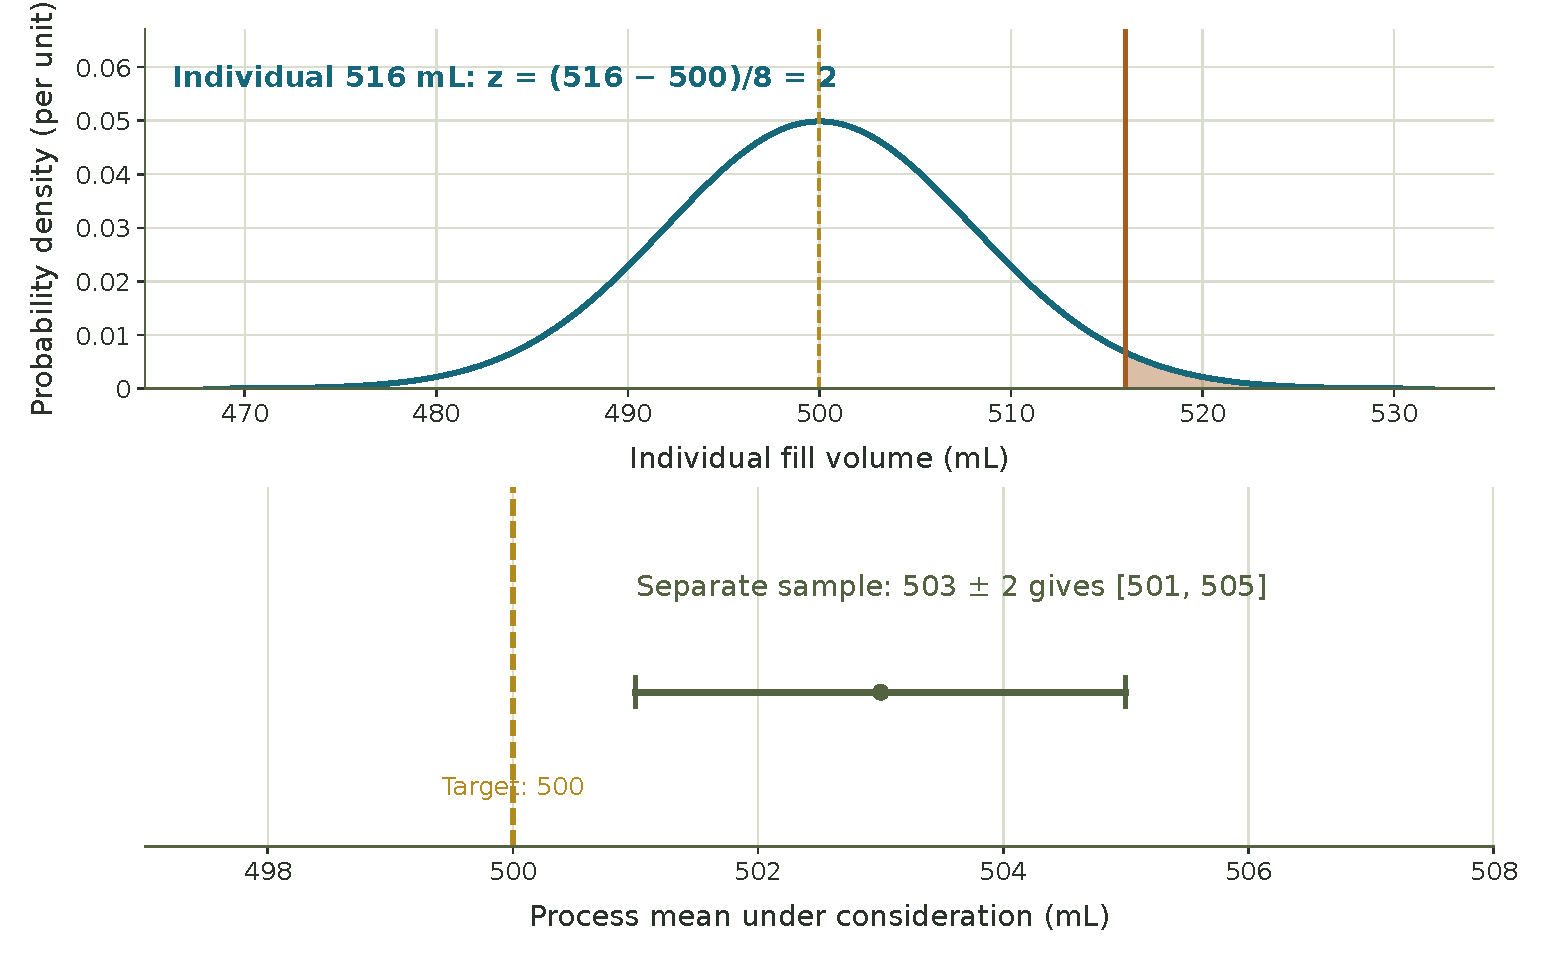
\includegraphics[width=\linewidth,height=3.4in,keepaspectratio]{../assets/week4/bottle-two-questions.pdf}
\captionof*{figure}{One graph describes bottle-to-bottle variation under a stated model. The other describes an estimate of the process mean from a separate sample.}
\end{minipage}\par\medskip

Statistical conclusions also depend on the population definition, selection method, measurement quality, and assumptions. State what was estimated and what the comparison supports. An interval alone does not identify a cause or justify a claim about every individual.


\begin{tcolorbox}[title={Pause and try 10},breakable]
A distribution has mean 60 and SD 12. An individual value is 78. A separate sample gives mean 63 with margin 3. Find the individual z-score and the sample interval. Does the interval contain 60?
\end{tcolorbox}

Week 5 uses measurements to choose actions in feedback systems. The distinction developed here remains essential: a noisy reading, a changing population mean, and an uncertain estimate are different reasons for what an observer sees.


References: NIST's \href{https://www.itl.nist.gov/div898/handbook/eda/section3/eda3661.htm}{normal distribution}, \href{https://www.itl.nist.gov/div898/handbook/eda/section3/eda352.htm}{confidence limits for a mean}, and \href{https://www.itl.nist.gov/div898/handbook/prc/section1/prc14.htm}{confidence-interval interpretation}. The chapter's core exercises supply their margins; calculating a t interval is outside the assigned arithmetic here.


\section*{Applications of the Same Distinctions}
\subsection*{A nutrition label and a planned larger sample}
A label claims a mean of 230 calories per serving. A random sample of 64 boxes has mean 243 and a reported margin of 8 calories. The supplied interval is
\[
[243-8,243+8]=[235,251]\text{ calories}.
\]
It excludes 230. This is a comparison of a proposed population mean with an interval estimate, not a conclusion about every individual serving or an explanation of the discrepancy.

For a planning comparison, increase the sample size to 256 while holding the confidence level, variability, design, and estimated center fixed. The planned margin becomes
\[
8\sqrt{64/256}=4,
\]
so the planned interval is $[239,247]$. An actual new sample could change the center as well as the estimated margin.

\begin{center}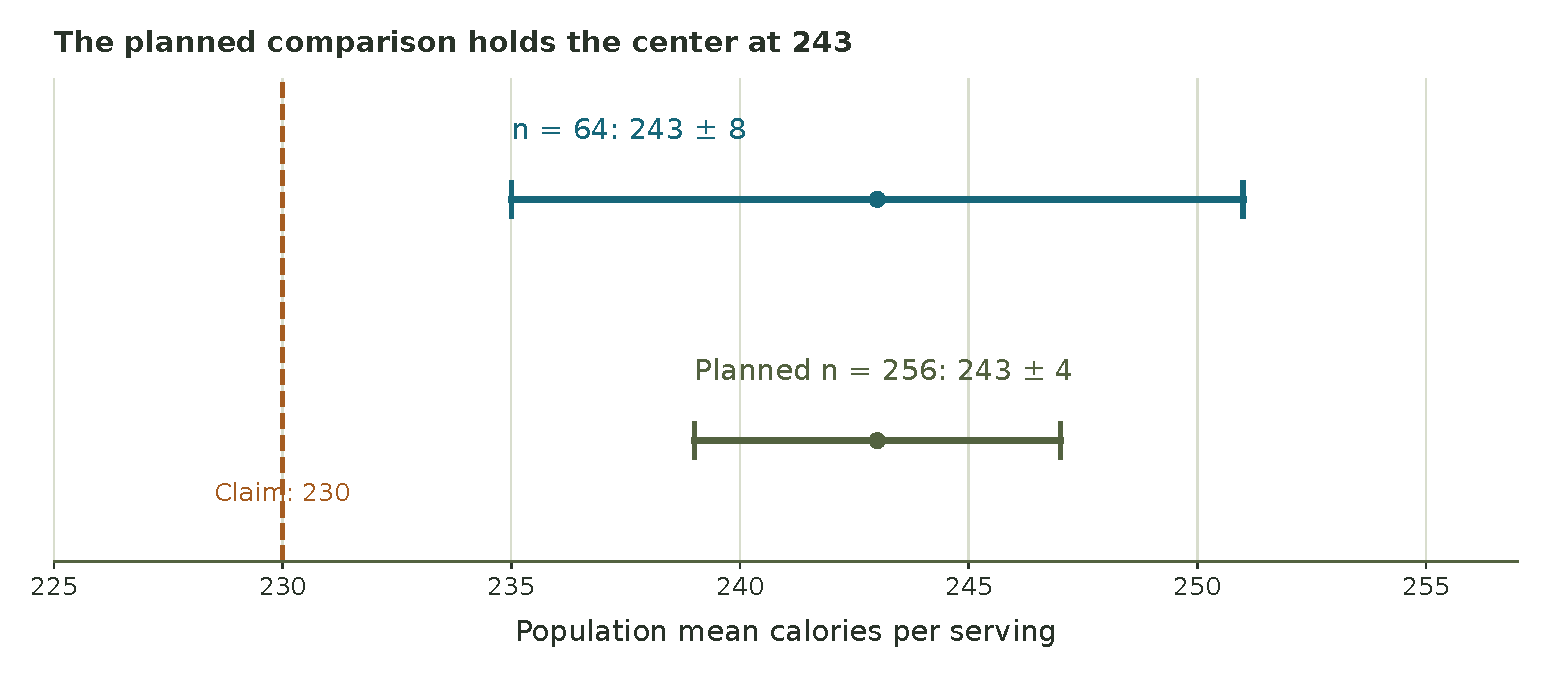
\includegraphics[width=\linewidth,height=2.8in,keepaspectratio]{../assets/week4/nutrition-intervals.pdf}\end{center}
The main application retains these calculations. A fuller interpretation also requires the population definition, selection method, measurement procedure, and the method used to obtain the reported margin.

\clearpage
\subsection*{A benchmark score is a sample statistic}
A hypothetical model answers 171 of 200 test questions correctly. Its observed accuracy is $171/200=0.855$, or 85.5\%. With a supplied margin of five percentage points, its reported interval is $[80.5\%,90.5\%]$, equivalently $[0.805,0.905]$.

\begin{center}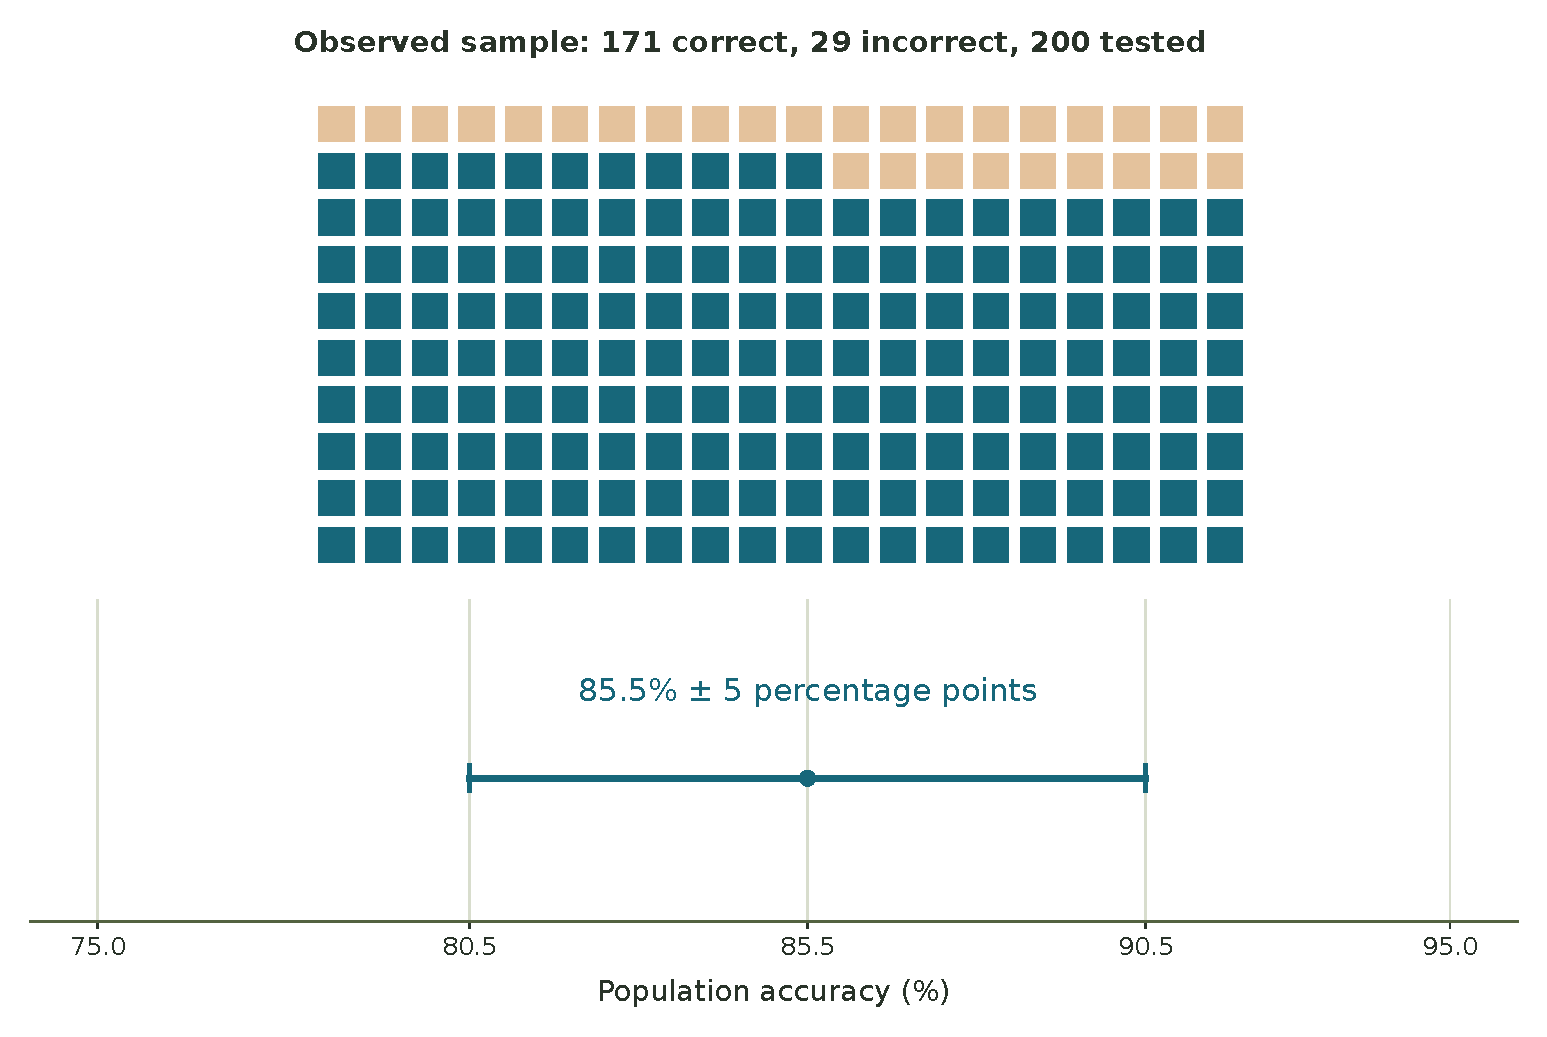
\includegraphics[width=\linewidth,height=3.5in,keepaspectratio]{../assets/week4/benchmark-estimate.pdf}\end{center}
The population is the defined collection of tasks that the sample can represent. This interval does not describe every possible request, every language, or every future answer. More data can reduce random sampling uncertainty without repairing an unrepresentative task collection or an inconsistent scoring rule.

Separate reported intervals also do not by themselves supply a formal test of a difference. Model A at $78\pm4$ and B at $80\pm4$ have overlapping intervals. That neither proves equality nor establishes superiority on every task. A suitable comparison may need task-level outcomes, especially if the same prompts were used for both models.

\clearpage
\section*{Chapter 4 Review}
For normal-region questions, use the Empirical Rule approximations unless stated otherwise. Retain signs and measurement units. For interval questions, use the reported margin; do not substitute the individual standard deviation for it. Explain the population quantity being estimated.
\begin{enumerate}
\item Apple weights are approximately normal with mean 180 g and SD 15 g. Find the percentage between 165 and 195, the percentage above 210, and both endpoints of the middle 95\%. For commute times with mean 35 minutes and SD 8 minutes, find the percentage between 19 and 51, the z-score of 59, and the percentage below 27.
\item A normal model has mean 50 and SD 6. Give the central one-, two-, and three-SD intervals. Estimate the percentage below 44 and between 38 and 62. Explain why the central percentages must not be added together.
\item For mean 100 and SD 15, find z-scores of 115, 85, 100, and 130. For mean 40 and SD 5, recover the raw values at z = 2, $-1$, 0.5, and $-3$. What does a negative z-score establish?
\item An athlete runs a mile in 400 seconds. Comparable times have mean 480 seconds and SD 60 seconds. Calculate and interpret the z-score. Why might a negative score be preferred in this setting? Does calculating z require the population to be normal?
\item Student A scores 520 on a test with mean 500 and SD 100. Student B scores 28 on a test with mean 21 and SD 5. Compare their standardized positions and explain the limit of comparing tests of different subjects. Separately, compare scores 88 with mean 80 and SD 10, and 74 with mean 65 and SD 6.
\item Identify the parameter and statistic in each study: (a) 1,200 voters surveyed, 58\% support; (b) 40 fish measured, mean length 31.2 cm; (c) 50 cereal boxes measured, mean weight 368 g. State why the sample count is not the target proportion or mean.
\item A school wants the mean number of books read per student in a year. Describe a simple random sample of 100 from 800 enrolled students. Explain one possible source of nonresponse or measurement bias. Would a larger biased sample automatically remove it?
\item Construct the supplied intervals for (a) 82 with margin 4; (b) 3.7 hours with margin 0.5; (c) 47\% with margin six percentage points. Give each full width and identify the units.
\newpage
\item A mean estimate is 4.2 hours with margin 0.3. Does its interval lie entirely above 4 hours? A poll estimates 38\% with margin four percentage points. Is a value above 40\% excluded? Does the interval establish that the population share is above 40\%? Distinguish compatibility from such a conclusion.
\item Use the original nutrition-label study: claim 230 calories, sample mean 243, reported margin 8, n = 64. Construct the interval and interpret the comparison. Plan a sample of 256 with other conditions and center fixed. Find its margin and interval. Explain what is assumed about the new center.
\item A study with n = 200 seeks half its current margin. Find the approximate required n. Starting from n = 100 and margin 10 units, calculate the planned margins at n = 200, 400, and 900. Name the quantities held fixed and explain why precision does not establish freedom from bias.
\item A distribution has mean 200 and SD 25. Locate the individual value 245 with a z-score. A separate sample of 50 produces mean 212 with reported margin 7. Construct its interval. Is the known model mean 200 included? Could a valid confidence procedure sometimes miss its target?
\item A distribution has mean 60 and SD 12. Is an individual value 78 within two SD? A separate sample of 80 has mean 63 and margin 3. Does its interval include 60? Explain why an endpoint counts as inside and why the two calculations address different questions.
\item For independent samples of size 25 from a normal population with mean 70 and known SD 10, compute the SE and the approximately 95\% known-SD margin using 1.96. A sample mean is 75; construct its interval and check 70. Must exactly 95\% of 50 intervals contain the mean? What stays fixed when the procedure is repeated?
\item Bulb lifetimes are approximately normal with mean 1,200 hours and SD 100. Estimate the percentage between 1,000 and 1,400, the percentage above 1,400, and the middle-68\% interval. Find and interpret z for 940. Separately, with mean 80 and SD 6, recover x at z = 2.5. Can the Empirical Rule alone give that cutoff's exact tail percentage?
\item A model answers 171 of 200 sampled tasks correctly. Give its decimal and percentage accuracy and its interval with a supplied five-percentage-point margin. What population could it estimate? Models A and B report mean scores $78\pm4$ and $80\pm4$. State what those reports show and what additional evidence could help compare their performance.
\end{enumerate}

\clearpage
{\setlength{\parskip}{4pt}\setlist{itemsep=5pt,topsep=3pt}
\section*{Solutions and Reasoning}

\paragraph{Short check 1.}
The process with the larger standard deviation. Equal centers do not imply equal spreads. A statement about an unknown distribution being ``normal'' still needs evidence or a stated modeling assumption.


\paragraph{Short check 2.}
Two standard deviations is 2 $\times$ 6 = 12. The interval is 50 $-$ 12 = 38 to 50 + 12 = 62. The interval is about individual values, not uncertainty about an estimated population mean.


\paragraph{Short check 3.}
Above $\mu$ + $\sigma$ is one tail: (100 $-$ 68)/2 = 16\%. Outside $\mu$ $\pm$ 2$\sigma$ includes both tails: 100 $-$ 95 = 5\%. Check whether the question requests one side or both.


\paragraph{Short check 4.}
The first z-score is (44 $-$ 50)/6 = $-$1: one standard deviation below the mean. For z = 2, x = 50 + 2(6) = 62. Location and percentage are different quantities.


\paragraph{Short check 5.}
The statistic is the sample mean 18.4 hours. Its target is the unknown mean lifetime of all batteries in the defined production population. The sample size is 100. A mean lifetime is not a count of tested batteries.


\paragraph{Short check 6.}
The mean's standard error is 12/\(\sqrt{36}\) = 2 units. The population standard deviation of individual measurements stays at 12 units. These answer different spread questions.


\paragraph{Short check 7.}
The interval is [3.2, 4.2] hours. Four is inside, so it is not excluded by this interval. Neither 3.7 nor the interval describes every individual observation.


\paragraph{Short check 8.}
No. Coverage is a long-run property; a finite run varies. In fact, 95\% of 50 is 47.5 intervals, which cannot be an observed count. Nor does a 95\% mean interval need to contain 95\% of individual observations.


\paragraph{Short check 9.}
Four times 200 gives 800. Doubling to 400 would instead multiply the margin by 1/\(\sqrt{2}\), about 0.707. A larger sample does not automatically repair bias.


\paragraph{Short check 10.}
The z-score is (78 $-$ 60)/12 = 1.5. The sample interval is [60, 66], so 60 is included at its lower endpoint. The z-score locates an individual; the interval estimates a population mean.


\clearpage

\subsection*{Chapter review: solutions}
\begin{enumerate}
\item Apple answers are about 68\%, about 2.5\%, and 150--210 g. The commute interval is $35\pm2(8)$, giving about 95\%. The value 59 has z = 3. Below 27 is below one SD under the mean, giving about 16\%. Tail answers use a complement followed by symmetry.
\item The intervals are [44,56], [38,62], and [32,68]. Below 44 is about 16\%; between 38 and 62 is about 95\%. The regions are nested: the 95\% region already includes the central 68\%, so adding those percentages would count the same outcomes repeatedly.
\item The z-scores are 1, $-1$, 0, 2. The recovered values are 50, 35, 42.5, 25. Negative z means below the mean. It does not require a negative original measurement and does not determine whether the outcome is desirable.
\item $z=(400-480)/60=-4/3\approx-1.33$. The time is about 1.33 SD below the comparable mean. A lower time means a faster run. Calculating z requires a finite mean and positive SD, not normality; using normal-tail percentages requires a suitable distributional assumption.
\item The original two scores give $z_A=0.2$, $z_B=1.4$, so B is farther above its own group's mean. The additional scores give 0.8 and 1.5, respectively. Relative position is not an absolute measurement of identical skills across different tests, nor a complete basis for judging a person.
\item (a) Parameter: population support proportion; statistic: 58\%. (b) Parameter: mean length in the defined fish population; statistic: 31.2 cm. (c) Parameter: mean box weight in the defined production population; statistic: 368 g. Counts 1,200, 40, and 50 describe how many units were observed, not the estimated mean or share.
\item Use a complete enrollment list with one identifier per student; select 100 distinct identifiers uniformly without replacement. Every subset of size 100 then has the same chance. Follow up consistently and define how books are counted. Nonresponse and recall or reporting errors can bias the result; collecting more observations by a biased procedure does not automatically remove that bias.
\item (a) [78,86], width 8 in the estimate's units. (b) [3.2,4.2] hours, width 1 hour. (c) [41\%,53\%], width twelve percentage points. Margin is half-width. A six-percentage-point adjustment differs from six percent of the estimate.
\newpage
\item The hours interval is [3.9,4.5], so it includes 4 and values below 4; it is not entirely above 4. The poll gives [34\%,42\%]. Values such as 41\% are compatible with that interval, but values at or below 40\% are also included. The interval therefore does not establish that the population share exceeds 40\%. Compare the full range, not only the point estimate.
\item The interval is [235,251] calories and excludes the claimed mean 230. Under the stated planning assumptions, $E_{\rm new}=8\sqrt{64/256}=4$, and the held-center interval is [239,247]. It also excludes 230. Keeping center 243 is an explicit comparison assumption, not a prediction of the next sample. Neither interval describes every individual box or identifies a cause of the discrepancy.
\item Required n is about 800. From baseline n = 100 and E = 10, planned margins are $10/\sqrt2\approx7.07$ at 200, 5 at 400, and $10/3\approx3.33$ at 900. The comparison keeps confidence, variability, and design comparable. Reduced random sampling variability does not correct an unrepresentative selection or a systematic measurement error.
\item The individual z-score is $(245-200)/25=1.8$. The sample interval is [205,219], which excludes the known model mean 200. That can occur even under a valid procedure: coverage below 100\% permits misses. A z-score describes an individual against the model; the interval comes from the separate observed sample.
\item $z=(78-60)/12=1.5$, so 78 is within two SD. The sample interval is [60,66], including 60 at its lower endpoint. Its endpoints are included in the supplied interval comparison. Neither the z-score nor this parameter interval substitutes for the other.
\item SE is $10/\sqrt{25}=2$ and margin is $1.96(2)=3.92$. The sample interval is [71.08,78.92], which misses 70. A set of 50 intervals need not have exactly 95\% coverage; 47.5 containing intervals is not even a possible count. The population parameter remains fixed while samples, means, and interval locations vary. Individual SD stays 10 when n changes.
\newpage
\item About 95\% lie between 1,000 and 1,400 hours; about 2.5\% lie above 1,400; the central 68\% spans 1,100--1,300 hours. For 940, $z=(940-1200)/100=-2.6$, or 2.6 SD below the mean. In the separate model, $x=80+2.5(6)=95$. The Empirical Rule provides no exact tail percentage at z = 2.5. Its one-tail approximations place that tail between the values at 2 and 3 SD; a normal-distribution calculation is needed for a more precise value.
\item Accuracy is $171/200=0.855=85.5\%$. Its supplied-margin interval is [80.5\%,90.5\%], or [0.805,0.905]. An appropriate population is a defined collection of tasks represented by the sample under the specified scoring conditions. A and B have intervals [74,82] and [76,84]; their point estimates differ by 2 and their intervals overlap. Overlap alone is not a formal test of the difference and does not prove equality. Task-level results, the relation between the two samples, and an interval or other suitable analysis for the performance difference could add evidence. No such mean comparison establishes a ranking on every task.
\end{enumerate}
\subsection*{References and activities}
The NIST Engineering Statistics Handbook provides accounts of the \href{https://www.itl.nist.gov/div898/handbook/eda/section3/eda3661.htm}{normal distribution}, \href{https://www.itl.nist.gov/div898/handbook/eda/section3/eda352.htm}{confidence limits for a mean}, and \href{https://www.itl.nist.gov/div898/handbook/prc/section1/prc14.htm}{confidence interpretation and known-SD intervals}. The online explorer uses repeated samples from a specified normal population to illustrate coverage; the laboratory's core interval questions use supplied margins.

The \href{https://bobovski66.github.io/MathInSociety/applications/week4_application.html}{nutrition-label application}, \href{https://bobovski66.github.io/MathInSociety/applications/week4_ai.html}{AI evaluation application}, and \href{https://bobovski66.github.io/MathInSociety/discussions/week4_discussion.html}{bottle-fill discussion} apply the same distinction between individual observations and estimated population quantities. Week 5 considers how measurements then guide actions in a feedback loop.
}
\end{document}
